\documentclass[aspectratio=169,12pt]{beamer}

% ------------------------------------------------------------
% Présentation Beamer (français) du papier arthritis_model_oliv.tex
% ------------------------------------------------------------
\usepackage[utf8]{inputenc}
\usepackage[T1]{fontenc}
\usepackage[french]{babel}
\usepackage{amsmath, amssymb}
\usepackage{graphicx}
\usepackage{tikz}
\usetikzlibrary{positioning, decorations.markings}
\usepackage{booktabs}

\graphicspath{{./}}

\usetheme{Madrid}
\usecolortheme{beaver}
\setbeamertemplate{navigation symbols}{}
\setbeamertemplate{footline}[frame number]
\setbeamertemplate{caption}[numbered]

\tikzset{
    mid arrow/.style={
        decoration={markings, mark=at position 0.5 with {\arrow{>}}},
        postaction={decorate}
    }
}

\title[Modèle mathématique de l'arthrite]{Modélisation mathématique de la polyarthrite rhumatoïde}
\subtitle{Un modèle minimal à quatre équations différentielles ordinaires}
\author[Azerad \textit{et al.}]{P.~Azerad, O.~Iosifescu, A.~Parmeggiani, O.~Bortolotti,\\ G.~Courties, F.~Apparailly}
\institute[IMAG -- IRMB -- L2C]{
IMAG, UMR5149, Université de Montpellier \\
L2C, UMR5221, Université de Montpellier \\
IRMB, UMR1183, Université de Montpellier, INSERM}
\date{\today}

\begin{document}

% ------------------------------------------------------------
\begin{frame}
\titlepage
\end{frame}

% ------------------------------------------------------------
\begin{frame}{Plan}
\tableofcontents
\end{frame}

% ==============================================================
\section{Contexte biologique}
% ==============================================================

\begin{frame}{Contexte~: la polyarthrite rhumatoïde}
\begin{itemize}
\item La polyarthrite rhumatoïde (PR) est une maladie auto-immune caractérisée par une inflammation chronique des articulations.
\item Modèle expérimental murin étudié ici~: le \alert{transfert de sérum arthritogène} (modèle STA, K/BxN), déclenché par une injection de sérum.
\item Ce signal externe active le système immunitaire et provoque une réponse inflammatoire dans le tissu synovial de l'articulation (membrane \emph{lining} L et \emph{sublining} SL).
\item Question~: pourquoi la crise inflammatoire se résorbe-t-elle parfois spontanément, et parfois se chronicise-t-elle~?
\end{itemize}
\end{frame}

\begin{frame}{Trois populations cellulaires clés}
\begin{itemize}
\item \textbf{Neutrophiles (N)}~: recrutés massivement et rapidement depuis le sang vers l'articulation enflammée ; dominants pendant la phase aiguë ; amplifient l'inflammation.
\item \textbf{Macrophages dérivés des monocytes (MoMac, M)}~: monocytes circulants recrutés dans l'articulation et différenciés en macrophages ; s'accumulent pendant la crise.
\item \textbf{Macrophages résidents sublining (SL-TRM, T)}~: forment une barrière protectrice et régulatrice ; \alert{progressivement déplétés} pendant les poussées inflammatoires.
\item Cette déplétion des SL-TRM coïncide avec l'accumulation des MoMac et des neutrophiles~: c'est ce phénomène que le modèle cherche à reproduire.
\end{itemize}
\end{frame}

\begin{frame}{État de l'art en modélisation mathématique}
{\footnotesize
\begin{itemize}\itemsep1pt
\item Domaine en forte croissance (plus de 200 publications/an en 2024) mais peu de modèles dédiés à la PR (Macfarlane \textit{et al.} 2020).
\item Modèles existants de la PR~:
  \begin{itemize}\itemsep0pt
  \item Seymour \& Anderson (2001)~: monocytes + cytokines IL-1, TNF-$\alpha$, IL-10.
  \item Baker \textit{et al.} (2013, 2017)~: cellules pro-/anti-inflammatoires, bifurcations.
  \item Friedman, Macfarlane \textit{et al.} (2022)~: modèles spatialisés (EDP), pannus.
  \end{itemize}
\item Inspiration principale~: Ciuperca \textit{et al.} (2024), maladie d'Alzheimer, modèle compartimental minimal à 5 équations.
\end{itemize}}
\vspace{1pt}
\begin{alertblock}{Notre approche}
\footnotesize Privilégier les \alert{populations cellulaires} plutôt que la cinétique des cytokines~: un modèle \textbf{minimal} (4 équations, 7 paramètres) isolant le paramètre adimensionnel clé de la transition inflammation aiguë $\to$ chronique.
\end{alertblock}
\end{frame}

% ==============================================================
\section{Le modèle mathématique}
% ==============================================================

\begin{frame}{Schéma du modèle}
\vspace{-4pt}
\begin{center}
\scalebox{0.66}{
\begin{tikzpicture}[node distance=4cm, auto, >=latex, thick]
    \node[draw, rectangle, fill=red!10, minimum width=3cm, minimum height=1cm] (N) {Neutrophiles $N$};
    \node[draw, rectangle, fill=green!10, minimum width=3cm, minimum height=1cm, right=of N] (M) {MoMac $M$};
    \node[draw, rectangle, fill=magenta!10, minimum width=3cm, minimum height=1cm, right=of M] (T) {SL-TRM $T$};
    \node[draw, circle, fill=blue!10, minimum size=2cm, below=of M, yshift=-1cm] (S) {Signal immun $S$};

    \draw[mid arrow, line width=1.5pt] (N) to[bend left=20] node[left, xshift=-2mm, yshift=2mm] {favorise $(a)$} (S);
    \draw[dashed,-|, line width=1.5pt] (T) to[bend left=20] node[right, xshift=2mm] {inhibition $(b)$} (S);
    \draw[mid arrow, line width=1.5pt] (S) to[bend left=20] node[left] {activation$(\alpha)$} (N);
    \draw[mid arrow, line width=1.5pt] (S) to[bend left=10] node[left,xshift=8mm, yshift=6mm] {activation $(\beta)$} (M);
    \draw[ dashed, line width=1.5pt, -|] (S) to[bend left=20] node[left, xshift=10mm, yshift=2mm] {inhibition $(\gamma)$} (T);
    \draw[ line width=1.5pt, loop above, looseness=8] (N) to node[above] {régulation $(\delta_N)$} (N);
    \draw[line width=1.5pt, loop above, looseness=8] (M) to node[above] {régulation $(\delta_M)$} (M);
    \draw[mid arrow, line width=1.5pt] (M.east) -- node[below, yshift=-2mm] {stimulation $(\delta_M)$} (T.west);
\end{tikzpicture}}
\end{center}
\small Les flèches pleines indiquent une activation, les flèches en tirets une inhibition.
\end{frame}

\begin{frame}{Le système d'équations}
Toutes les variables sont \alert{adimensionnées} par rapport à leur valeur de référence à l'état sain (baseline).
\begin{align*}
\frac{dS}{dt} &= (a\, N - b\,T)\, S \\[4pt]
\frac{dN}{dt} &= \alpha\, S\, N - \delta_N\, N (N-1) \\[4pt]
\frac{dM}{dt} &= \beta\, S - \delta_M\, M (M-1) \\[4pt]
\frac{dT}{dt} &= -\gamma\, S\, T + \delta_M\, M (1-T)
\end{align*}
avec $a,b,\alpha,\beta,\gamma,\delta_N,\delta_M > 0$.
\end{frame}

\begin{frame}{Interprétation biologique des équations}
\begin{itemize}
\item \textbf{Signal $S$}~: amplifié par les neutrophiles (facteur $a$), inhibé par les SL-TRM (facteur $b$).
\item \textbf{Neutrophiles $N$}~: recrutés par le signal $S$ (facteur $\alpha$) ; terme logistique $\delta_N N(N-1)$ ramenant $N$ vers sa valeur de base en l'absence d'inflammation.
\item \textbf{MoMac $M$}~: recrutement \emph{linéaire} en $\beta S$ (indépendant de $M$ lui-même, car limité par le réservoir sanguin) ; même type de régulation logistique.
\item \textbf{SL-TRM $T$}~: détruits par le signal (taux $\gamma S$) ; terme $\delta_M M (1-T)$~: les MoMac \alert{restaurent} $T$ quand il est déplété, mais l'\alert{inhibent} s'il est en excès.
\item En résumé~: l'inflammation \emph{augmente} $N$ et $M$, mais \emph{diminue} $T$.
\end{itemize}
\end{frame}

\begin{frame}{Positivité et bornes des solutions}
\begin{block}{Existence et positivité}
Le théorème de Cauchy-Lipschitz garantit l'existence locale d'une solution. Le champ de vecteurs étant \emph{quasi-positif}, toute solution partant de conditions initiales positives reste positive pour tout $t\geq 0$ (Haraux, 2016).
\end{block}
\begin{block}{Bornes}
\begin{itemize}
\item $T(t) \le \max(1, T(0))$ pour tout $t$ (via le lemme de Gronwall)~: les SL-TRM restent bornés par leur niveau basal.
\item $M(t) \ge \min(1, M(0))$ et $N(t) \ge \min(1, N(0))$~: les réservoirs sanguin/médullaire garantissent une borne inférieure.
\item En revanche $S$, $N$, $M$ ne sont \emph{pas nécessairement bornés} au cours du temps~: le modèle est pertinent pour la \alert{dynamique de crise}, pas le comportement en temps long.
\end{itemize}
\end{block}
\end{frame}

% ==============================================================
\section{Points d'équilibre}
% ==============================================================

\begin{frame}{Points d'équilibre~: mise en équations}
Les équilibres $(S^*,N^*,M^*,T^*)$ annulent le second membre~:
\begin{align*}
(a N^* - b T^*)\,S^* &= 0 \\
\alpha S^* N^* - \delta_N N^* (N^*-1) &= 0 \\
\beta S^* - \delta_M M^* (M^*-1) &= 0 \\
-\gamma S^* T^* + \delta_M M^* (1-T^*) &= 0
\end{align*}
\vspace{4pt}
\textbf{Équilibre sans inflammation} ($S^*=0$)~: le point \alert{biologiquement pertinent} est
\[
(S^*,N^*,M^*,T^*) = (0,1,1,1) \quad \text{(état sain)}.
\]
D'autres équilibres existent avec $N^*=0$ ou $M^*=0$~: non pertinents biologiquement (populations cellulaires jamais nulles in vivo) et instables.
\end{frame}

\begin{frame}{Équilibres inflammatoires ($S^*>0$)~: réduction à une cubique}
En éliminant $N^*$, $S^*$ et $M^*$ en fonction de $T^*$, l'équation restante pour $T^*$ se ramène à une \alert{équation cubique}~:
\[
{(T^*)}^3 + \frac{A}{C}\left(1-B-C\right)(T^*)^2 + \frac{A}{C}\left(2B-1\right) T^* - \frac{AB}{C} = 0
\]
\begin{itemize}
\item Remarquable~: alors que le système dépend de 7 paramètres, les équilibres ne dépendent que de \alert{3 paramètres adimensionnels} $A$, $B$, $C$.
\item Les racines positives $T^*$ de cette cubique donnent ensuite $N^*, S^*, M^*$ via
\[
N^* = \tfrac{b}{a}T^*, \quad S^* = \tfrac{\delta_N}{\alpha}\left(\tfrac{b}{a}T^*-1\right), \quad M^* = 1-\tfrac{\beta}{\gamma}+\tfrac{\beta}{\gamma T^*}.
\]
\end{itemize}
\end{frame}

\begin{frame}{Trois paramètres adimensionnels}
\[
A = \frac{a}{b}, \qquad B = \frac{\beta}{\gamma}, \qquad C = \frac{\gamma\,\delta_N}{\alpha\,\delta_M}
\]
\begin{itemize}
\item $A$~: rapport entre l'effet \alert{pro-inflammatoire} des neutrophiles et l'effet \alert{anti-inflammatoire} des SL-TRM.
\item $B$~: rapport entre le taux de recrutement des MoMac et le taux de destruction des SL-TRM par le signal.
\item $C$~: rapport entre les paramètres de régulation logistique des MoMac et des neutrophiles.
\end{itemize}
\bigskip
\begin{alertblock}{Résultat clé}
C'est le paramètre $A = a/b$ qui s'avère \textbf{déterminant} pour le devenir de la crise inflammatoire.
\end{alertblock}
\end{frame}

\begin{frame}{Nombre de racines positives et faisabilité biologique}
\begin{columns}
\begin{column}{0.55\textwidth}
\begin{itemize}
\item \emph{Règle des signes de Descartes}~: selon les signes de $B+C-1$ et $B-\tfrac12$, la cubique admet 1 ou 3 racines positives.
\item \textbf{Faisabilité}~: il faut de plus $S^*\ge 0$, $M^*\ge 0$, soit
\[
T^* \ge A \quad \text{et (si $B>1$)} \quad T^*\le \tfrac{B}{B-1}.
\]
\item Résultat central~: pour $A>1$, \textbf{aucune} racine n'est faisable ; pour $A<1$, il existe \textbf{exactement une} racine faisable $T^*\in(A,1)$.
\end{itemize}
\end{column}
\begin{column}{0.45\textwidth}
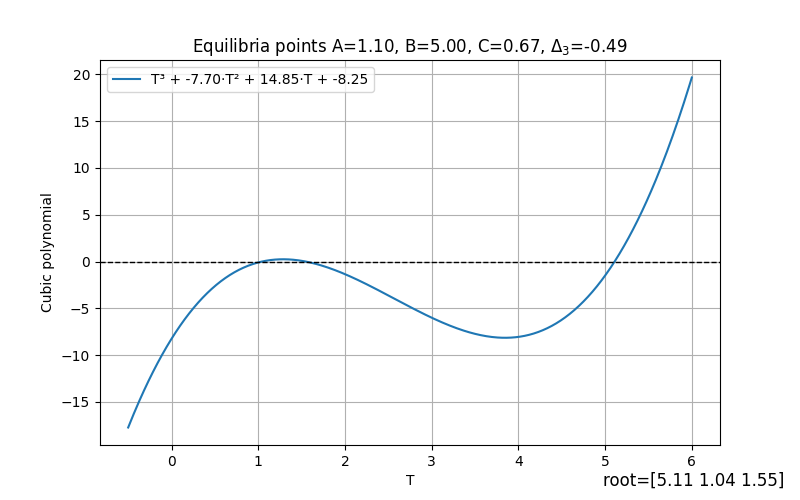
\includegraphics[width=\linewidth]{three_roots.png}
\end{column}
\end{columns}
\end{frame}

% ==============================================================
\section{Stabilité et bifurcation}
% ==============================================================

\begin{frame}{Stabilité de l'équilibre sans inflammation}
Au point $(0,1,1,1)$, la matrice jacobienne est triangulaire par blocs et ses valeurs propres sont
\[
a-b, \qquad -\delta_N, \qquad -\delta_M, \qquad -\delta_M.
\]
\begin{itemize}
\item Les trois dernières sont toujours négatives.
\item Seul le signe de $a-b$ compte~: l'équilibre sain est
\begin{itemize}
\item \textbf{stable} si $A=a/b < 1$ (guérison spontanée possible),
\item \textbf{instable} si $A = a/b > 1$ (inflammation persistante).
\end{itemize}
\item Cas critique $A=1$~: valeur propre nulle $\Rightarrow$ analyse de la \emph{variété centrale} (Perko, 2001). On montre que la variété centrale est \alert{répulsive}~: l'équilibre sain est donc instable dès $A=1$.
\end{itemize}
\end{frame}

\begin{frame}{Stabilité des équilibres inflammatoires}
\begin{itemize}
\item Pour l'unique équilibre inflammatoire faisable (qui n'existe que si $A<1$), on étudie le polynôme caractéristique $P(\lambda)$ de degré 4 du jacobien.
\item En utilisant $M^*>1$, $T^*<1$ (conséquences des équations d'équilibre) et à nouveau la règle de Descartes, on montre que $P(\lambda)$ admet \textbf{exactement une racine positive}.
\end{itemize}
\begin{alertblock}{Conclusion}
L'équilibre inflammatoire, lorsqu'il existe ($A<1$), est \textbf{toujours instable}.
\end{alertblock}
\begin{itemize}
\item Ainsi, pour $A<1$~: le système bascule entre l'attracteur sain (stable) et cet équilibre instable qui joue le rôle de \alert{seuil} (séparatrice) entre guérison et crise persistante.
\end{itemize}
\end{frame}

\begin{frame}{Diagramme de bifurcation}
\begin{columns}
\begin{column}{0.5\textwidth}
\begin{itemize}
\item Une unique bifurcation a lieu en $A=1$ (type \emph{transcritique})~:
\begin{itemize}
\item $A<1$~: équilibre sain stable + équilibre inflammatoire instable (séparatrice).
\item $A\ge 1$~: équilibre sain instable, \textbf{plus aucun} équilibre biologiquement faisable.
\end{itemize}
\item Interprétation~: franchir $A=1$ fait disparaître toute possibilité de retour à l'état sain.
\end{itemize}
\end{column}
\begin{column}{0.5\textwidth}
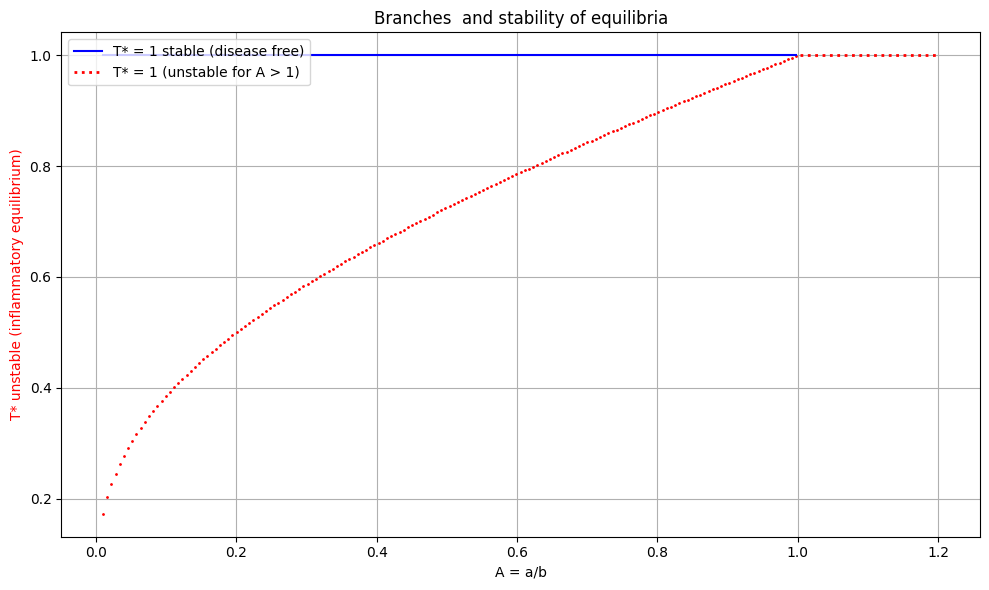
\includegraphics[width=\linewidth]{bifurcation.png}
\end{column}
\end{columns}
\end{frame}

% ==============================================================
\section{Simulations numériques}
% ==============================================================

\begin{frame}{Scénario de base~: rémission ou chronicisation~?}
Paramètres~: $\alpha=\beta=\gamma=\delta_N=\delta_M=1$, $b=1$, conditions initiales $S(0)=N(0)=M(0)=T(0)=1$, durée 20 jours.
\begin{columns}
\begin{column}{0.5\textwidth}
\centering $A=0.35$ (guérison)\\
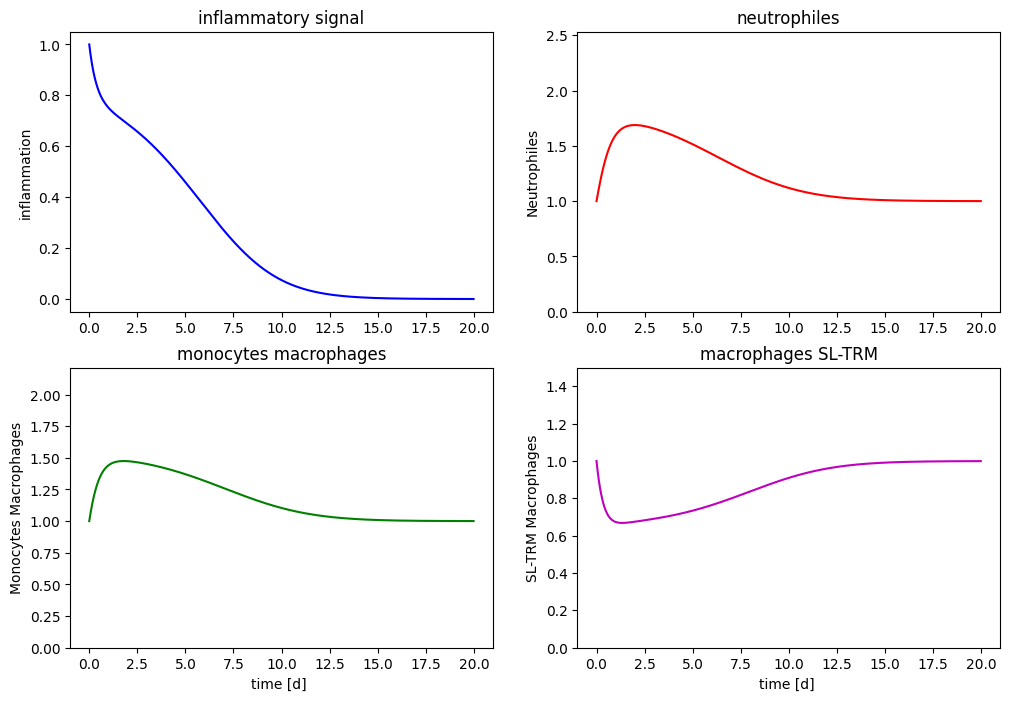
\includegraphics[width=\linewidth]{A=0,35.png}
\end{column}
\begin{column}{0.5\textwidth}
\centering $A=0.38$ (chronicisation)\\
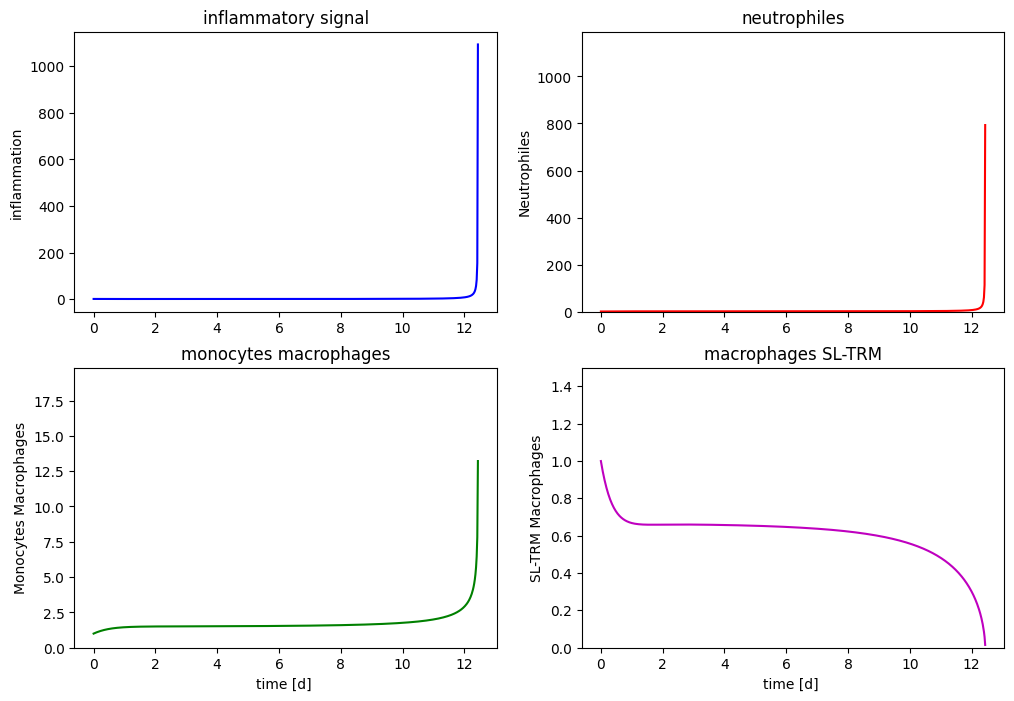
\includegraphics[width=\linewidth]{A=0,38.png}
\end{column}
\end{columns}
\vspace{4pt}
\small Une variation infime de $A=a/b$ (0.35 vs 0.38) suffit à faire basculer le pronostic.
\end{frame}

\begin{frame}{Rôle de la dose initiale et de l'état des SL-TRM}
\begin{columns}
\begin{column}{0.5\textwidth}
\centering\small $A=0.38$, $S(0)=0.5$\\ (demi-dose~: guérison)\\
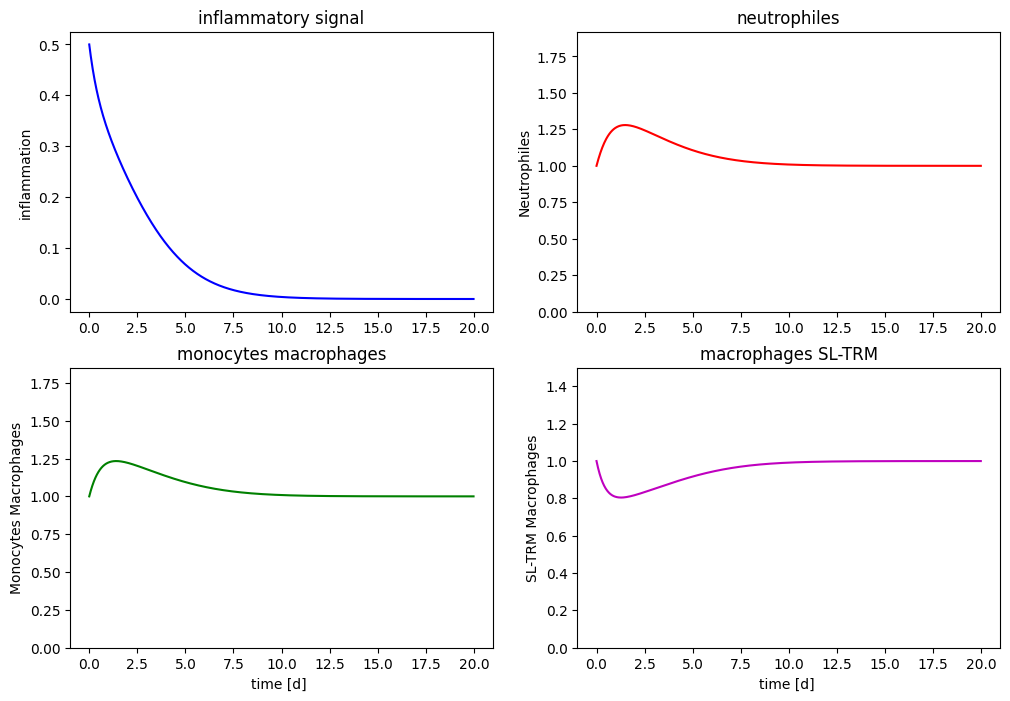
\includegraphics[width=0.92\linewidth]{A=0,38_S0=0,5.png}
\end{column}
\begin{column}{0.5\textwidth}
\centering\small $A=0.35$, $T(0)=0.5$\\ (SL-TRM déplétés~: chronicisation)\\
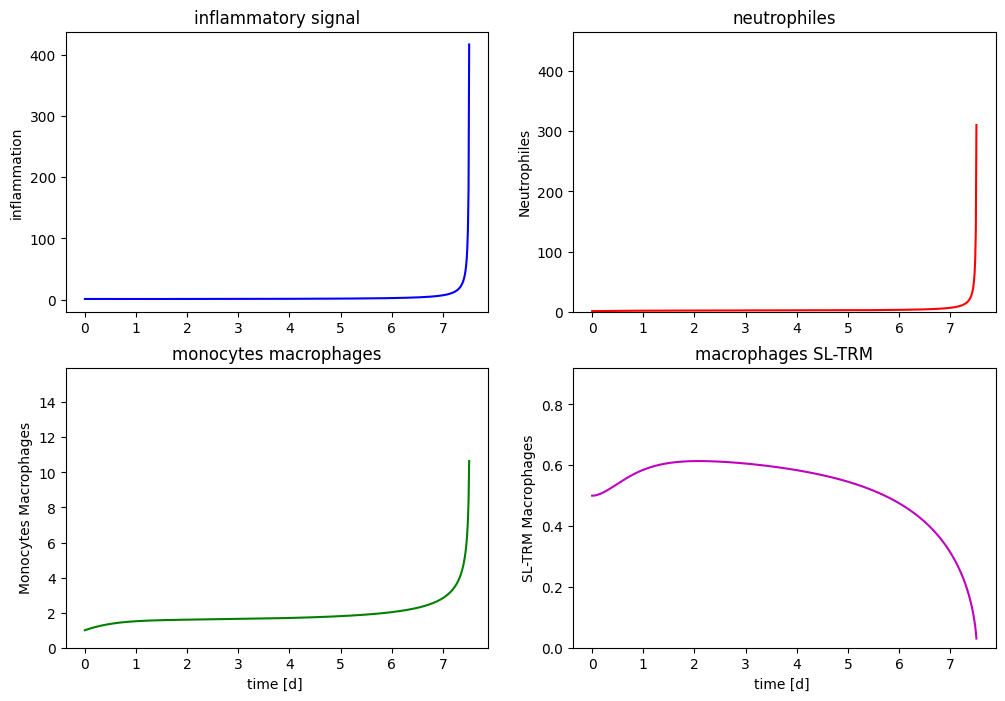
\includegraphics[width=0.92\linewidth]{A=0,35_T=0,5.png}
\end{column}
\end{columns}
\vspace{2pt}
{\footnotesize
\begin{itemize}
\item Même avec $A<1$, un déficit initial en SL-TRM peut faire basculer vers la crise persistante.
\item Réduire la dose initiale $S(0)$ peut, à l'inverse, suffire à éviter la chronicisation.
\end{itemize}}
\end{frame}

\begin{frame}{Renforcer la régulation~: effet de $\delta_M$}
\begin{columns}
\begin{column}{0.5\textwidth}
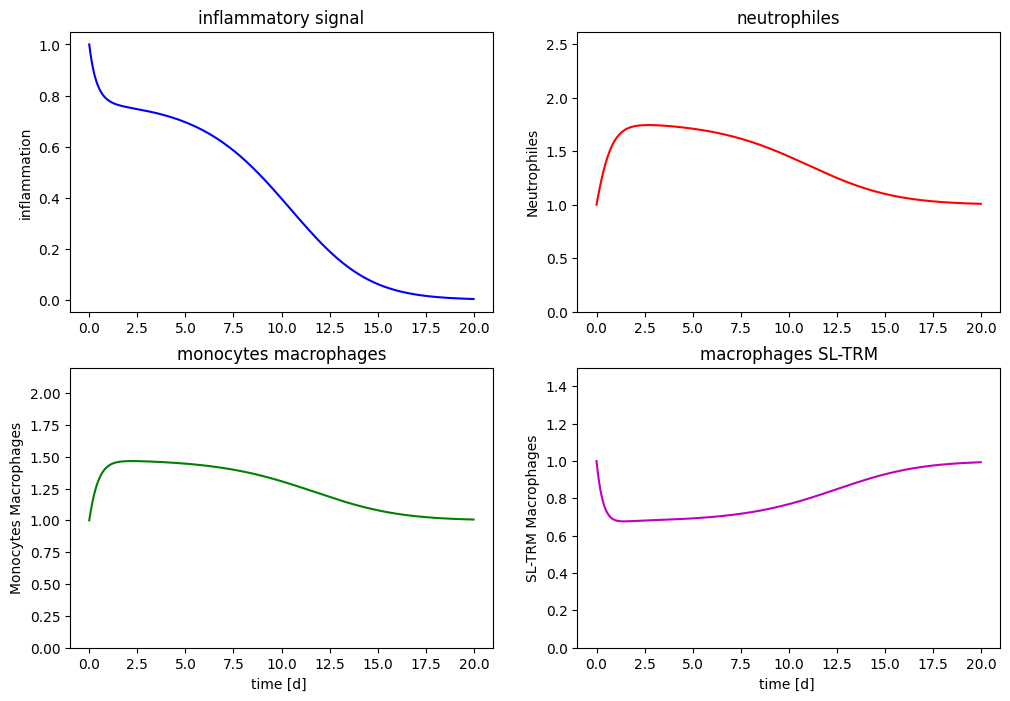
\includegraphics[width=\linewidth]{A=0,38_delta_M=1,1.png}
\end{column}
\begin{column}{0.5\textwidth}
\begin{itemize}
\item Reprise du cas chronicisant $A=0.38$.
\item En augmentant légèrement $\delta_M$ (de 1 à 1.1)~: renforcement de la régulation MoMac~$\leftrightarrow$~SL-TRM.
\item Résultat~: le système \alert{revient} à l'équilibre sain.
\item Piste thérapeutique~: agir sur la régulation des macrophages pourrait suffire à résoudre la crise.
\end{itemize}
\end{column}
\end{columns}
\end{frame}

\begin{frame}{Carte de pronostic dans le plan $(A, S(0))$}
\begin{columns}
\begin{column}{0.5\textwidth}
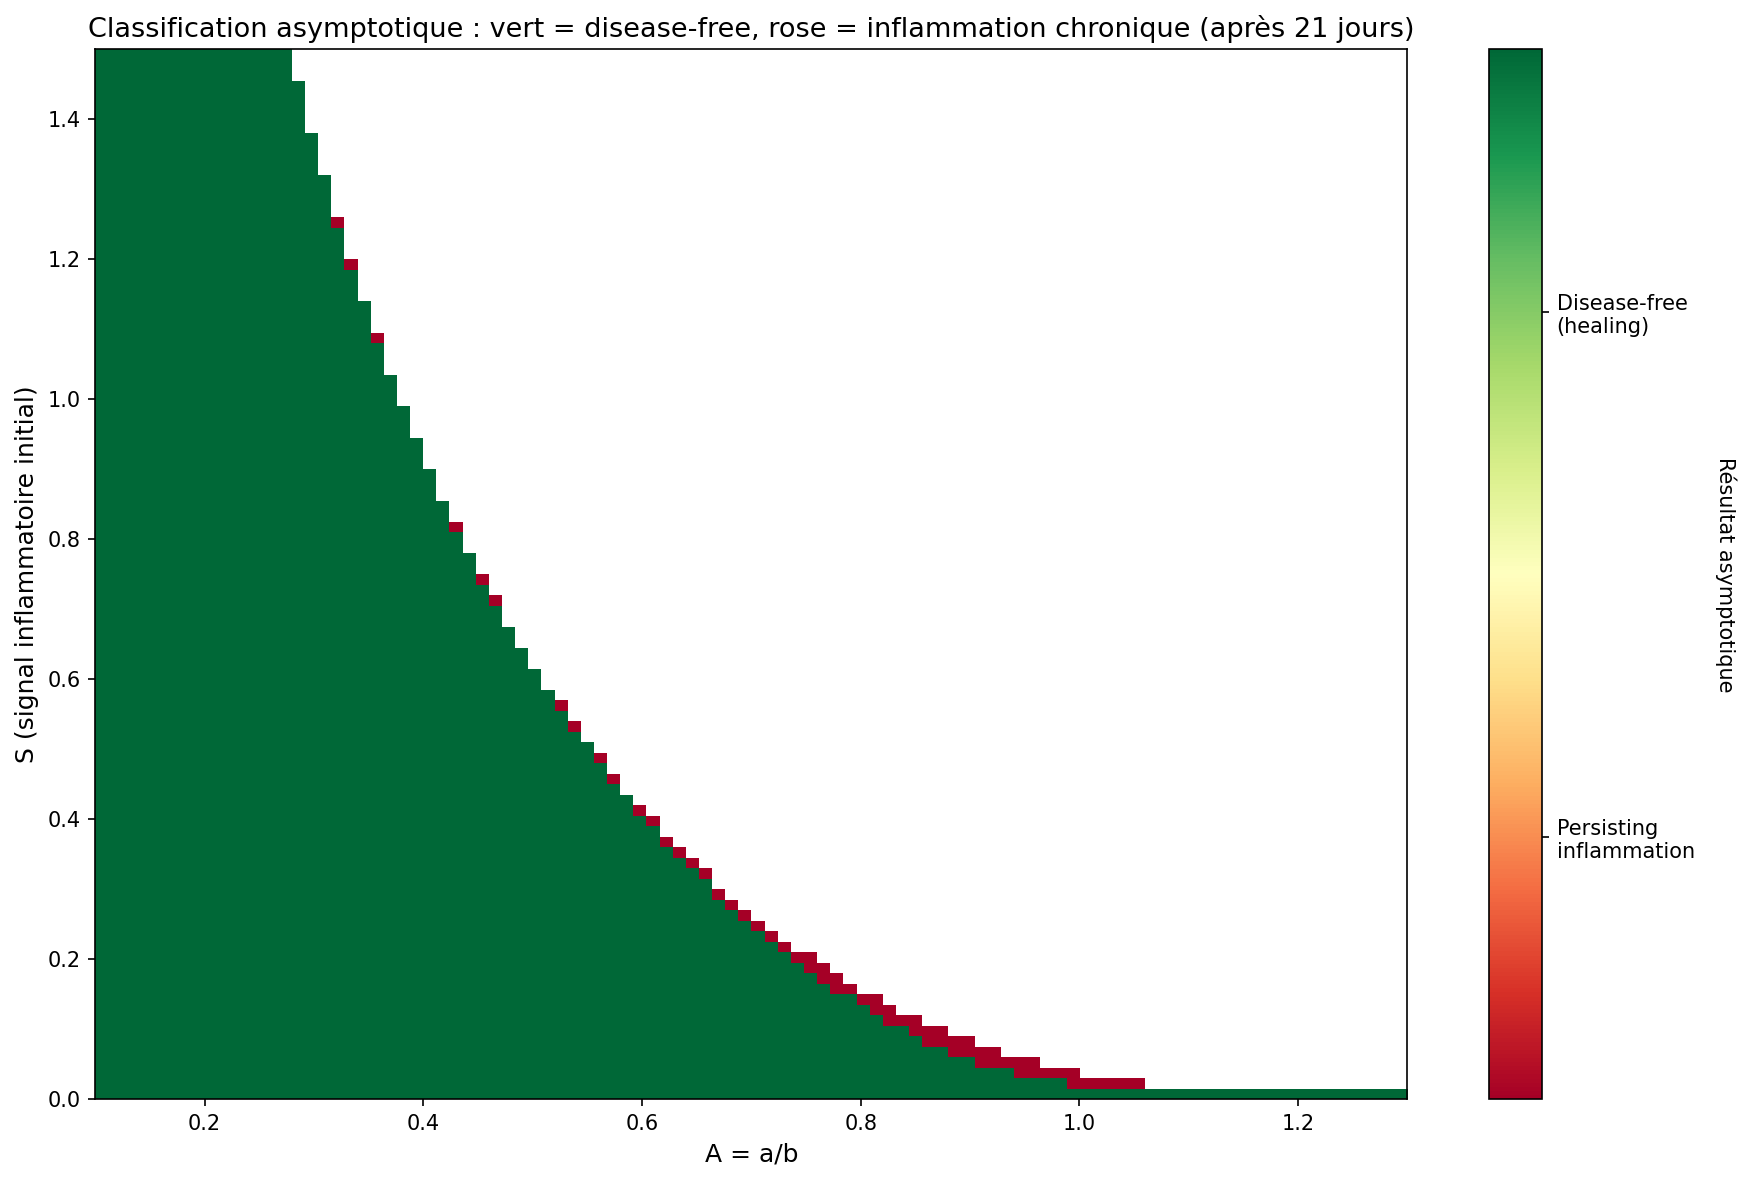
\includegraphics[width=\linewidth]{phase_plane_classification.png}
\end{column}
\begin{column}{0.5\textwidth}
{\footnotesize
\begin{itemize}
\item Pour chaque couple $(A, S(0))$~: simulation sur 3 semaines, classification \textcolor{green!50!black}{guérison} / \textcolor{red}{chronicité} ($\pm 5\%$ autour de l'état sain).
\item Pour $A<1$~: il existe un \alert{seuil de dose} $S(0)$ en dessous duquel le système guérit toujours ; ce seuil \emph{augmente} quand $A$ diminue.
\item Pour $A\ge 1$~: chronicisation systématique, quelle que soit la dose initiale, même très faible.
\item Exemple~: avec $S(0)=5$, le système guérit encore pour $A=0.072$ mais plus pour $A=0.073$~: une variation infime de $A$ suffit à inverser le pronostic.
\end{itemize}}
\end{column}
\end{columns}
\end{frame}

% ==============================================================
\section{Discussion et conclusion}
% ==============================================================

\begin{frame}{Prédictions biologiques testables}
\begin{itemize}
\item Le devenir de la crise d'arthrite expérimentale (STA) dépendrait d'un \alert{équilibre} entre amplification inflammatoire (neutrophiles) et régulation par les macrophages résidents (SL-TRM).
\item Le modèle prédit l'existence d'un \textbf{seuil} séparant inflammation auto-résolutive et arthrite persistante.
\item Ce seuil peut être déplacé par~:
  \begin{itemize}
  \item l'intensité du stimulus arthritogène initial,
  \item l'efficacité du recrutement des monocytes/MoMac,
  \item l'intégrité du compartiment des macrophages résidents (SL-TRM).
  \end{itemize}
\item Tests proposés~: quantification temporelle de N, M, T pendant la STA ; perturbations réduisant le recrutement des neutrophiles ou préservant/renforçant les SL-TRM.
\end{itemize}
\end{frame}

\begin{frame}{Conclusion et perspectives}
\begin{itemize}
\item Un modèle \alert{minimal} (4 équations, 7 paramètres) reproduit les traits essentiels de la dynamique MoMac / neutrophiles / SL-TRM lors d'une poussée inflammatoire articulaire.
\item Un \textbf{unique paramètre critique} $A=a/b$ gouverne les rétroactions positives/négatives en jeu~: rapport entre effet pro-inflammatoire des neutrophiles et effet protecteur des SL-TRM.
\item Implication thérapeutique~: des traitements agissant \emph{différentiellement} sur les neutrophiles et sur les macrophages résidents SL-TRM pourraient être efficaces contre l'arthrite.
\item \textbf{Perspectives}~: estimation des paramètres à partir de données expérimentales, extension du modèle à l'évaluation de stratégies thérapeutiques (contrôle optimal), analyse de sensibilité.
\end{itemize}
\end{frame}

\begin{frame}{Remerciements et références}
\vspace{-6pt}
{\footnotesize
\begin{block}{Remerciements}
\footnotesize Institut Universitaire Hospitalier Immun4Cure, « Institute for innovative immunotherapies in autoimmune diseases » [France 2030/ANR-23-IHUA-0009].
\end{block}
\vspace{-4pt}
\begin{block}{Quelques références}
\footnotesize
\begin{itemize}\itemsep0pt
\item Culemann S. \textit{et al.} (2019), \textit{Nature}, 572, 670--675.
\item Christensen A.D. \textit{et al.} (2016), \textit{Front. Immunol.}, 7, 213.
\item Ciuperca I. \textit{et al.} (2024), \textit{R. Soc. Open Sci.}, 11, 231536.
\item Ugolkov Y. \textit{et al.} (2024), \textit{Front. Immunol.}, 15, 1371620.
\end{itemize}
\end{block}
\vspace{-4pt}
\begin{block}{Code et données}
\footnotesize Notebook Jupyter (Python) des simulations~: \url{https://github.com/azerad/immunomath}
\end{block}}
\end{frame}

\end{document}
